\documentclass{standalone}

\usepackage{tikz}
\usepackage{pgfplots}

\usetikzlibrary{calc}

\begin{document}
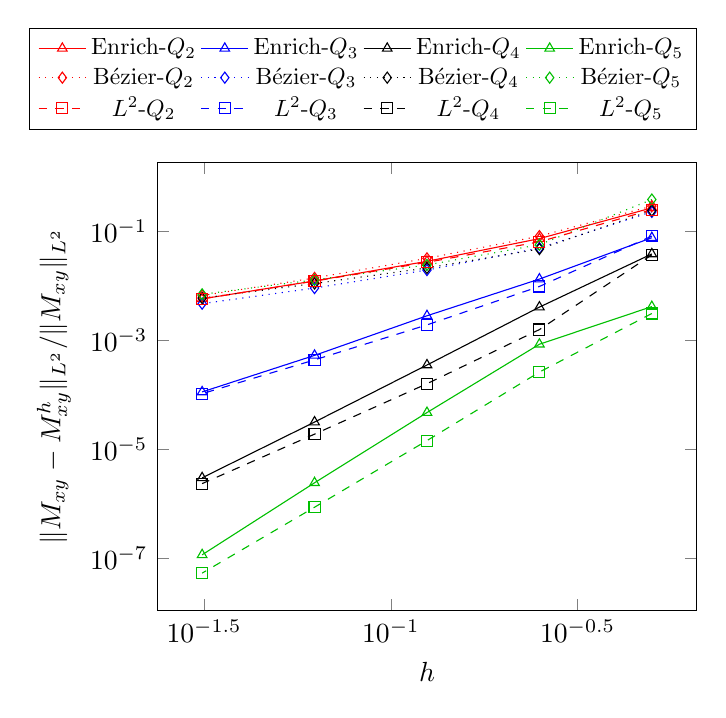
\begin{tikzpicture}
    \begin{loglogaxis}[
        legend columns=4,
    	legend style={at={(1,1.3)}, nodes={scale=.85, transform shape}},
        xlabel=$h$,
        ylabel=${\|M_{xy}-M_{xy}^{h}\|_{L^2}}/{\|M_{xy}\|_{L^2}}$ 
    ]

    \addplot [color=red,mark=triangle] plot coordinates {

        (.5,        0.270831)
        (.25,       0.0738606)
        (.125,      0.0283063)
        (.0625,     0.0123702)
        (0.03125,   0.00579056)
    };

    \addplot [color=blue,mark=triangle] plot coordinates {

        (.5,        0.0767154)
        (.25,       0.0133629)
        (.125,      0.00283569)
        (.0625,     0.000531652)
        (0.03125,   0.000113495)
    };

    \addplot [color=black,mark=triangle] plot coordinates {

        (.5,        0.0386826)
        (.25,       0.00408515)
        (.125,      0.000354129)
        (.0625,     3.1772e-05)
        (0.03125,   3.0114e-06)
    };

    \addplot [color=green!75!black,mark=triangle] plot coordinates {

        (.5,        0.00417627)
        (.25,       0.000851431)
        (.125,      4.74623e-05)
        (.0625,     2.44174e-06)
        (0.03125,   1.16354e-07)
    };

    
    \addplot [color=red,mark=diamond, every mark/.append style={solid}, dotted] plot coordinates {

        (.5,        0.291843)
        (.25,       0.0821029)
        (.125,      0.0320999)
        (.0625,     0.0140305)
        (0.03125,   0.00664538)
    };

    
    \addplot [color=blue,mark=diamond, every mark/.append style={solid}, dotted] plot coordinates {

        (.5,        0.228918)
        (.25,       0.0496135)
        (.125,      0.0195823)
        (.0625,     0.00915261)
        (0.03125,   0.00472855)
    };

    \addplot [color=black,mark=diamond, every mark/.append style={solid}, dotted] plot coordinates {


        (.5,        0.242685)
        (.25,       0.0475542)
        (.125,      0.0213917)
        (.0625,     0.0110885)
        (0.03125,   0.00599046)
    };

    \addplot [color=green!75!black,mark=diamond, every mark/.append style={solid}, dotted] plot coordinates {

        (.5,        0.385542)
        (.25,       0.0572021)
        (.125,      0.024297)
        (.0625,     0.012922)
        (0.03125,   0.00702619)
    };


    \addplot [color=red,mark=square, every mark/.append style={solid}, dashed] plot coordinates {

        (.5,        0.250862)
        (.25,       0.0646643)
        (.125,      0.0271181)
        (.0625,     0.0122579)
        (0.03125,   0.00579306)
    };

    
    \addplot [color=blue,mark=square, every mark/.append style={solid}, dashed] plot coordinates {

        (.5,        0.082199)
        (.25,       0.00978504)
        (.125,      0.00192879)
        (.0625,     0.000439429)
        (0.03125,   0.000105379)
    };

    \addplot [color=black,mark=square, every mark/.append style={solid}, dashed] plot coordinates {

        (.5,        0.0372113)
        (.25,       0.00158214)
        (.125,      0.000160703)
        (.0625,     1.90781e-05)
        (0.03125,   2.35645e-06)
    };

    \addplot [color=green!75!black,mark=square, every mark/.append style={solid}, dashed] plot coordinates {

        (.5,        0.00312188)
        (.25,       0.000262489)
        (.125,      1.45223e-05)
        (.0625,     8.69177e-07)
        (0.03125,   5.36776e-08)
    };


    \logLogSlopeTriangle{0.16}{0.075}{0.06}{4}{green!75!black};
    \logLogSlopeTriangle{0.16}{0.075}{0.26}{3}{black};
    \logLogSlopeTriangle{0.16}{0.075}{0.46}{2}{blue};
    \logLogSlopeTriangle{0.16}{0.075}{0.67}{1}{red};

    \legend{Enrich-$Q_2$\\Enrich-$Q_3$\\Enrich-$Q_4$\\Enrich-$Q_5$\\B\'ezier-$Q_2$\\B\'ezier-$Q_3$\\B\'ezier-$Q_4$\\B\'ezier-$Q_5$\\$L^2$-$Q_2$\\$L^2$-$Q_3$\\$L^2$-$Q_4$\\$L^2$-$Q_5$\\}
    \end{loglogaxis}
\end{tikzpicture}

\end{document}
